%chapter experiment results
\chapter{Experiment Results \& Justification}
This section is based on lessons learned and any observations made in section \ref{implwhirlpool}.

\section{HTTP Fetch URL}
\begin{figure}[h!]
  \centering
  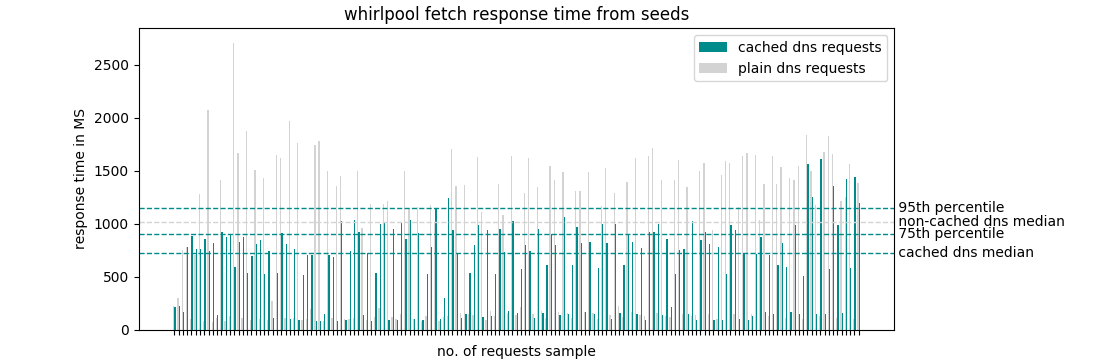
\includegraphics[width=18cm,height=12cm,keepaspectratio]{../media/crawler/dns_response_time.png}
  \caption{HTTP request latencies for a sample of N request across seeds}
  \label{fig:dnsresponse}
\end{figure}

\noindent
The HTTP fetcher subsystem is responsible for downloading the HTML page for a given absolute URL. Figure
\ref{fig:dnsresponse} present a grouped bar chart combining HTTP requests with DNS lookup entries cached
and non-cached. Each bar is a HTTP call to the web host and height of the bar is the time taken to respond 
back to a corresponding request. The graphs shows median response time for cached and non-cached DNS
lookups. It also shows response time for 75th and 95th percentiles for cached DNS lookups. Overall,
comparing both the medians, HTTP request with cached DNS entries performed faster by approx. 250ms compared to non-cached requests. There are far fewer cached requests exceeding the 95th percentile compared to
plain requests.
\pagebreak

\section{RabbitMQ Dashboard}
Following statistics are derived using the management plugin available to monitor and handle active
rabbitmq node. 

\begin{figure}[h!]
  \centering
  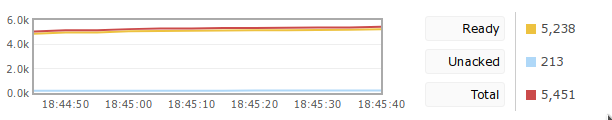
\includegraphics[width=16cm,height=10cm,keepaspectratio]{../media/crawler/rmq_queued_messages.png}
  \caption{Queued messages}
  \label{fig:qmsg}
\end{figure}

\noindent
The line graph in figure \ref{fig:qmsg} shows 5,236 messages are ready to be delivered across various
consumers connected to this rabbitmq instance with 213 messages are yet to be acknowledged by consumers
itself as messages are manually acknowledged through custom logic between consumer to consumer processes.

\begin{figure}[h!]
  \centering
  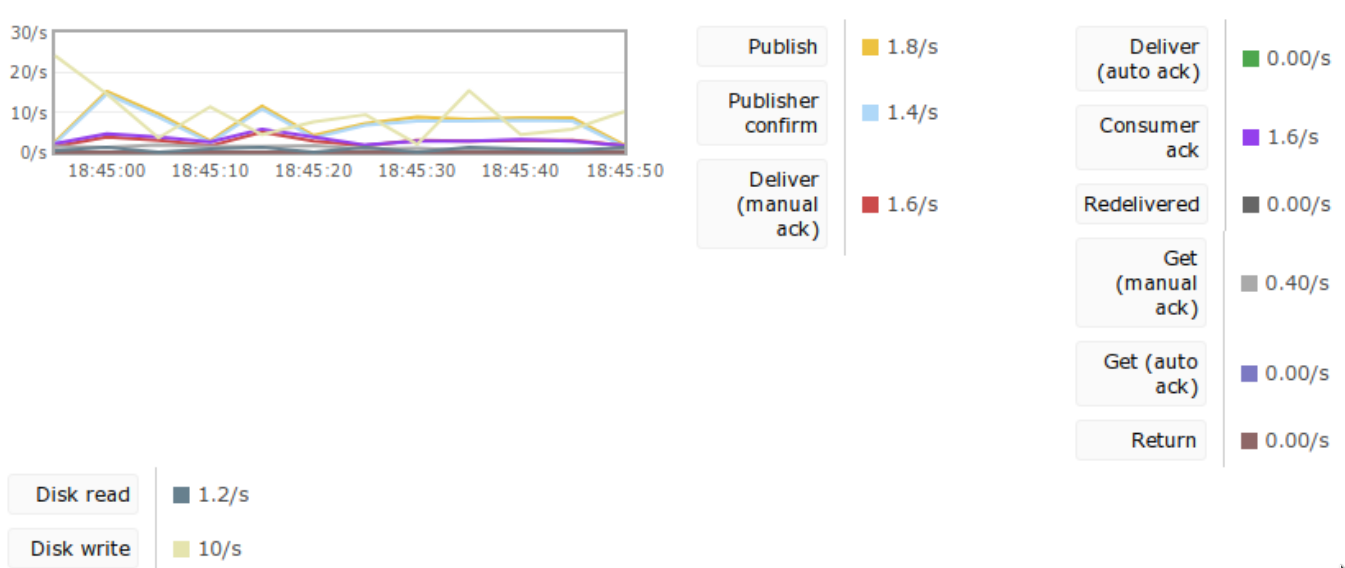
\includegraphics[width=16cm,height=12cm,keepaspectratio]{../media/crawler/rmq_msg_rates.png}
  \caption{Message Rates}
  \label{fig:msgrates}
\end{figure}

\noindent
Figure \ref{fig:msgrates} measures various operations/sec occurring on the work queues for the given rabbitmq instance. Publish is the rate at which messages enter the work queue. Message Delivery with manual
acknowledgement is the rate at which messages are delivered to the consumer(s). Publisher confirms is the
rate at which rabbitmq is confirming messages published by the producer. Since the consumer carries out
the processing of the message compared to the producer, the consumer rate is slower by 200 ms to that of
producer.

\pagebreak

\noindent
Figure \ref{fig:rmqnode} shows total number of connections open on that instance.
Every connection consumes memory mainly the connections TCP buffer. The number of open client connections and rate at which connection open/close aid in determining issues common in messaging systems like connection leaks and high connection churn.
These issues eventually lead to exhausting resources in which it wont accept new
client connections from that point onward. With this, memory consumption and socket count turns red. 

\begin{figure}[h!]
  \centering
  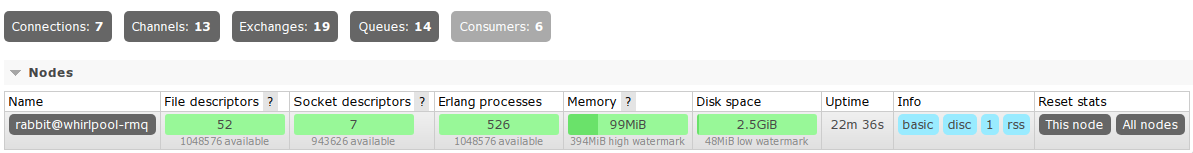
\includegraphics[width=16cm,height=10cm,keepaspectratio]{../media/crawler/rmq_node.png}
  \caption{RMQ node}
  \label{fig:rmqnode}
\end{figure}

\noindent
Connection leaks can be learned from the following chart from rabbitmq management
dashboard under file and socket descriptors where number of connections keep growing. For this project, figure \ref{fig:process_stats} shows stable sockets on the node.

\begin{figure}[h!]
  \centering
  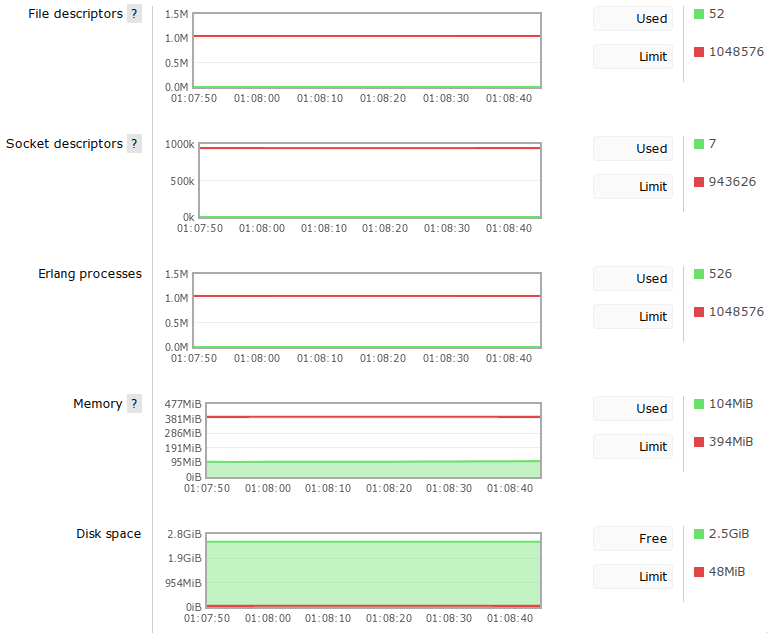
\includegraphics[width=14cm,height=18cm,keepaspectratio]{../media/crawler/process_stats.png}
  \caption{File and Socket descriptors}
  \label{fig:process_stats}
\end{figure}

\pagebreak

\noindent
Below are long-lived connections to the rabbitmq node using language specific client
library used by the subsystem of the crawler. The client are using plain authentication to connect to virtual host(vhost) of the RMQ node. The connection churn rate
is observed only during the crawler bootup indicating the clients use long-lived
connections, figure \ref{fig:churn_stats}.

\begin{figure}[h!]
  \centering
  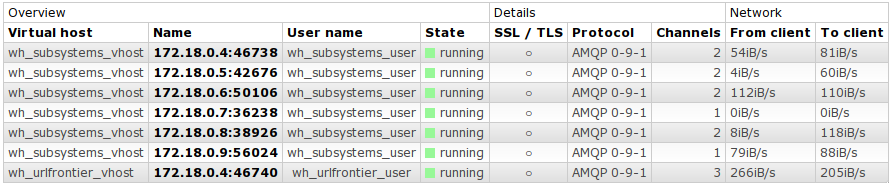
\includegraphics[width=16cm,height=10cm,keepaspectratio]{../media/crawler/rmq_connections.png}
  \caption{RMQ Connections}
  \label{fig:rmqconn}
\end{figure}

\begin{figure*}[h!]
    \centering
    \begin{subfigure}
        \centering
        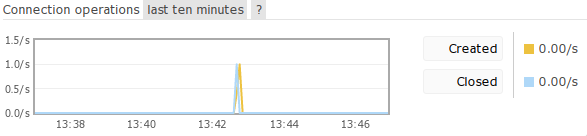
\includegraphics[width=3in, height=1.2in]{../media/crawler/churn_stats_conn.png}
    \end{subfigure}%
    ~ 
    \begin{subfigure}
        \centering
        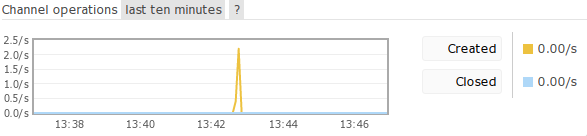
\includegraphics[width=3in, height=1.2in]{../media/crawler/churn_stats_channel.png}
    \end{subfigure}
    \caption{churn rate}
    \label{fig:churn_stats}
\end{figure*}

\noindent
Channels in message queues are lightweight connections sharing a single TCP connection. The channels only exist in context of a connection. A consumer using threads/processes to process messages maintains new channel per thread or a process. The channels are never shared between them. Figure \ref{fig:rmqchannel} shows single digit
channels opened by each whirlpool subsystem. Figure \ref{fig:rmqnode} on previous
page shows total count of channels for the given RMQ instance.

\begin{figure}[h!]
  \centering
  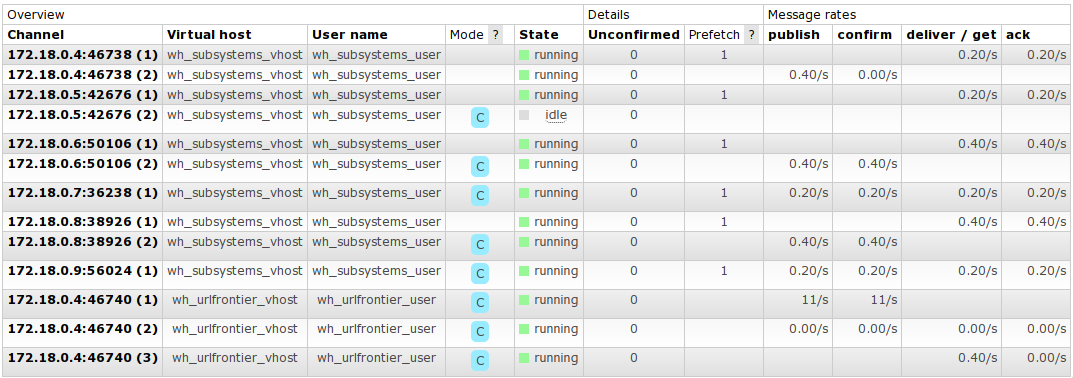
\includegraphics[width=16cm,height=8cm,keepaspectratio]{../media/crawler/rmq_channels.png}
  \caption{RMQ Channels}
  \label{fig:rmqchannel}
\end{figure}

\noindent
Channels also face similar bottlenecks discussed about RMQ connections when metrics
on opening/closing of channels appear to be unusual. The churn rate for the channels
in this project is very low and in fact negligible and that is only due to long-lived connections.

\pagebreak

\section{Content SeenTest: Near Duplicate Detection}\label{handle_dedupe}
\noindent
In Summary, when it comes to detecting similarity between two web pages using shingling, the pages are converted into bag of phrases. The challenge lies in storage requirements because the word size for a phrase $p$ adds a space complexity of O$(np)$, where $n$ is no. of times we have to save the document. Applying a hash function outputs a integer and is able to improve space complexity of bag of phrases to O$(n)$. Minhash\cite{dedupe} brings storage requirement to O$(1)$ but time complexity of query documents is O$(n)$. Simhashing\cite{dedupe} performs better than Minhash by querying on a fix $q$ sorted list of hashes. Its time complexity is given as O$(q * log(n))$.
\\
\\
To achieve the time complexity expressed in previous paragraph, simhash can be
combined with Locality-Sensitive Hashing(LSH)\cite{lsh} which is a technique that
can quickly find similar entries in a large pool of data. This technique is
classified under randomized algorithms which do not guarantee exact answer but
through a probability function outputs an answer close to it. The function can be
tuned to set the cutoff high/low or as desired.
\\
\\
\noindent
For near-duplicate detection at scale, LSH hashes similar documents into same bucket groups that have
a probability threshold set. The bucket count is much smaller than number of documents need to be
compared. As this technique maps a range of similar documents to same buckets, the number of
comparison operations is greatly reduced. The hash collisions are encouraged and are maximized differing
from minimum collision probability that exist in cryptographic hash functions.

\pagebreak

\section{Hash based rebalancing}
\begin{figure}[h!]
  \centering
  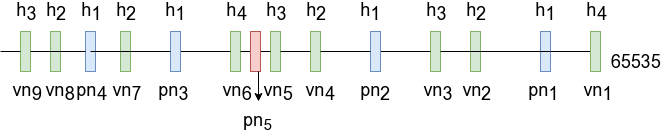
\includegraphics[width=12cm,height=5cm,keepaspectratio]{../media/crawler/addingnode.png}
  \caption{adding new node to existing cluster of nodes}
  \label{fig:addingnode}
\end{figure}

\noindent
Key observation while rebalancing a cluster when adding or removing a node like $pn_5$:
\begin{itemize}
  \item entire vnodes are moved between pnodes
  \item number of vnodes present do not change 
  \item assignment of hash of urls to vnodes do not change
  \item only the assignment of vnodes to pnodes is changed
\end{itemize}

\noindent
The maximum number of pnodes that can be provisioned to manage scalability is equal to total number of
vnodes. At some point if the crawler process changes its property from being just a topical crawler to
also be comprehensive, its compute capacity can get overhauled, thus requiring more horizontal scalability.
Determining how many machines the crawler can outgrow to depends on what needs to be accomplished with the crawler.

\pagebreak

\section{MongoDB documents}
NoSQL stores are a good choice for unstructured data like in figure \ref{fig:mongo_data}. The
dimensionality of the data needs to be expanded to cater to data mining and machine learning.

\begin{figure}[h!]
  \centering
  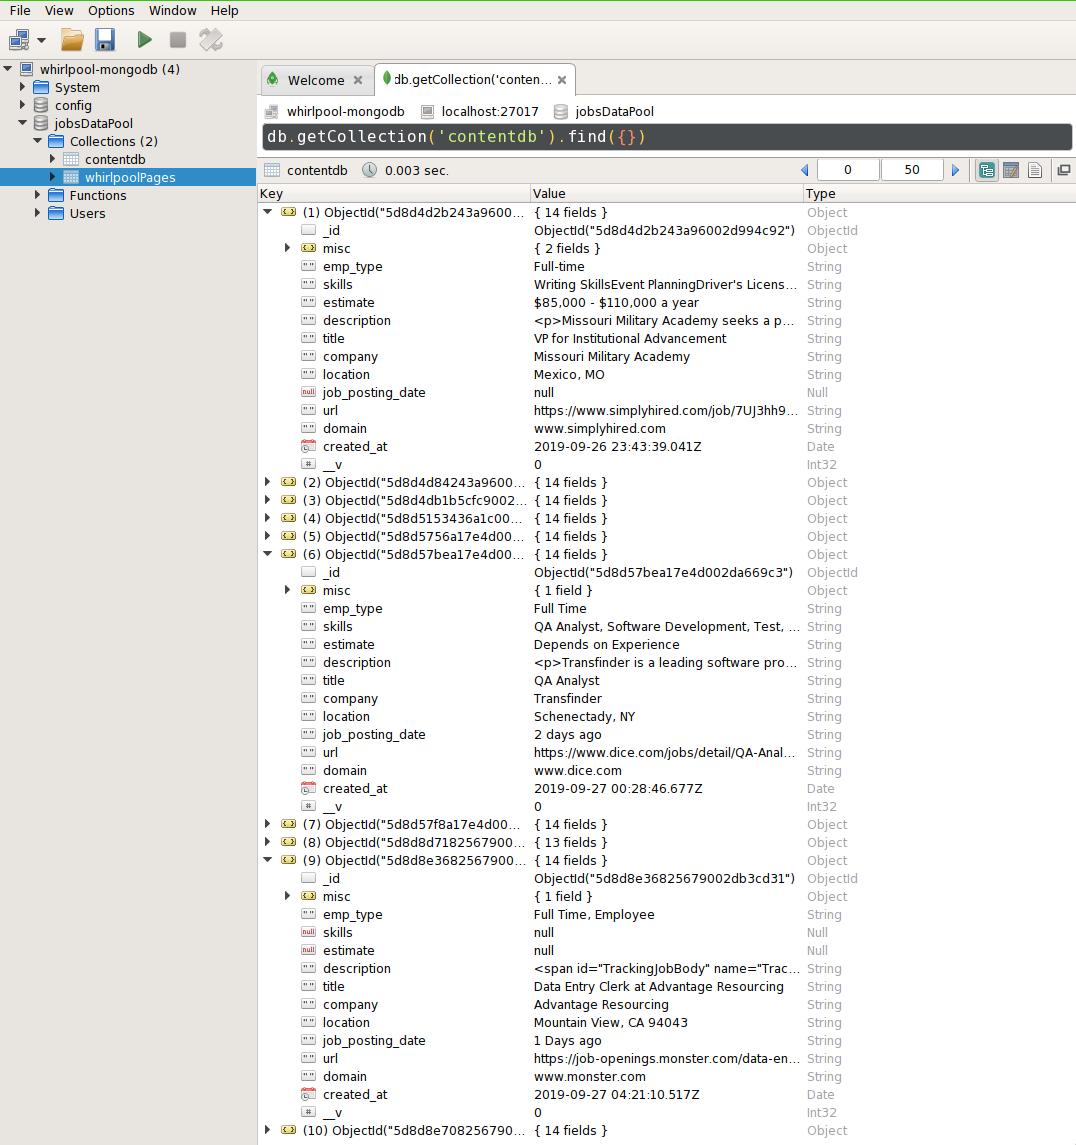
\includegraphics[width=12cm,height=18cm,keepaspectratio]{../media/crawler/collecteddata.png}
  \caption{screenshot of collected data through crawler}
  \label{fig:mongo_data}
\end{figure}
\pagebreak

%\section{Postgres ContentSeen \& DUE Fingerprints}

\pagebreak

\section{Whirlpool as a Microservice Architecture}
\emph{microservices.io} defines microservices as a 
\begin{quote}
  "architectural style that structures an application as a collection of services that
  are:
  \begin{itemize}
    \item Highly maintainable and testable
    \item Loosely coupled
    \item Independently deployable
    \item Organized around business capabilities
    \item Owned by a small team
  \end{itemize}
  "
\end{quote}
The Whirlpool crawler project in this thesis shares similar characteristics. Its implementation is a
event-driven microservice identified by the use of asynchronous, broker-based messaging for collaboration
between services(subsystems).
\\
\\
There exist 2 ways to communicate between microservices:
\begin{itemize}
\item \underline{Synchronous} - where each service calls directly other service and awaits reply.
  This is achieved using REST or gRPC. Note that this results in dependency between the two. 
\item \underline{Asynchronous} - a message queue is used as a separate layer to send message from
  service A to service B. Principles of message queue(covered in section \ref{eventdriven} apply here)
  where service A doesn't wait for the reply.
\end{itemize}

With message broker
\begin{itemize}
\item the messages get delivered with at least once durability
\item ensures the workflow cycle completes when participants are temporarily unavailable
\item ordered delivery
\item mechanism for scaling consumers
\item easier to diversify language runtimes
\end{itemize}

\pagebreak